\subsection*{Mean Average Precision}

Um die Genauigkeit von Objektdetektoren zu messen, wird oft die Metrik \textit{mean Average Precision} (mAP) gewählt. Diese setzt sich aus zwei grundlegenden Größen zusammen \cite{JonathanHui.20180307}):

\begin{equation} \label{precisionandrecall}
\begin{split}
Precision = \frac{True Positive}{True Positive + False Positive} \\
\\
Recall = \frac{True Positive}{True Positive + False Negative}
\end{split}
\end{equation}
\equations{Precision und Recall}

\textit{Precision} sagt also etwas über die Verlässlichkeit einer Klassifikation aus während \textit{Recall} Aussagen über die Erkennungsfähigkeit eines Objektdetektors trifft. Wichtig ist es hierbei anzumerken, dass mehrfach detektierte Objekte nur einmal als positiver Befund aufgefasst werden, die restlichen Detektionen gehen als \textit{False Positives} \cite{TarangShah.20180127}.

\begin{figure}[ht]
	\begin{center}
		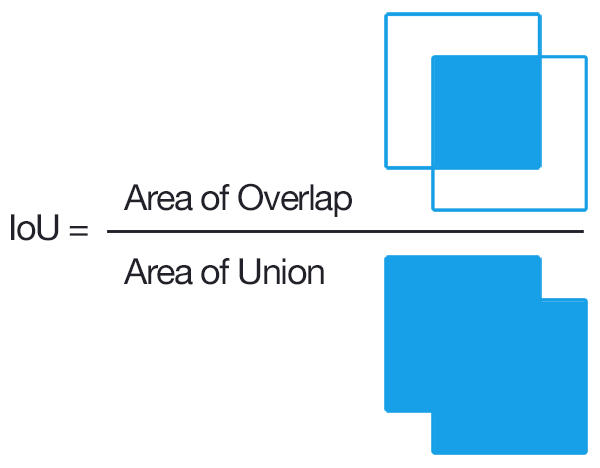
\includegraphics[width=8cm]{Bilder/iou_equation.png} 
		\caption[Intersection over Union]{Intersection over Union \cite{AdrianRosebrock.20161107}}
		\label{iou}
	\end{center}
\end{figure}

Die Klassifikation, ob eine Bounding Box das gewünschte Objekt enthält und demnach ein positiver Fall vorliegt, wird anhand eines sogenannten \textit{Intersection over Union} (IoU) Schwellwertes bestimmt (siehe Abbildung \ref{iou}). Er beschreibt ein Maß der Überdeckung der detektierten Bounding Box zur wahren Bounding Box und wird auch als \textit{confidence score} bezeichnet. Für den kompletten Datensatz werden nun für unterschiedliche \textit{confidence scores} jeweils \textit{Precision} und \textit{Recall} bestimmt und anschließend in einem Graphen aufgetragen. Meistens werden die \textit{confidence scores} so gewählt, sodass sich eine äquidistante Abstufung in den \textit{Recall} Werten ergibt \cite{TarangShah.20180127}. 

\begin{figure}[ht]
	\subfigure{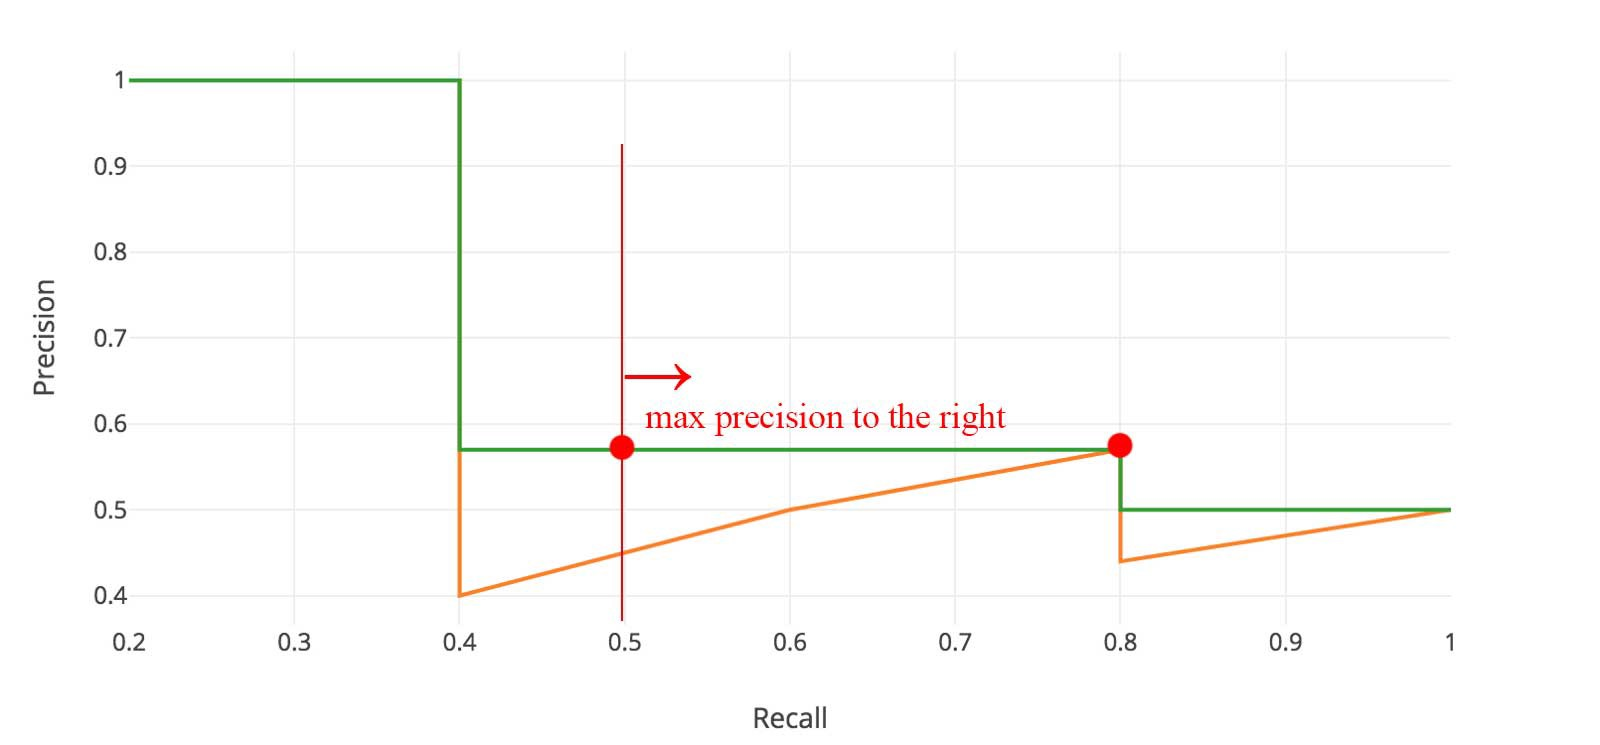
\includegraphics[width=12cm]{Bilder/map_graph1.png}} 
	\subfigure{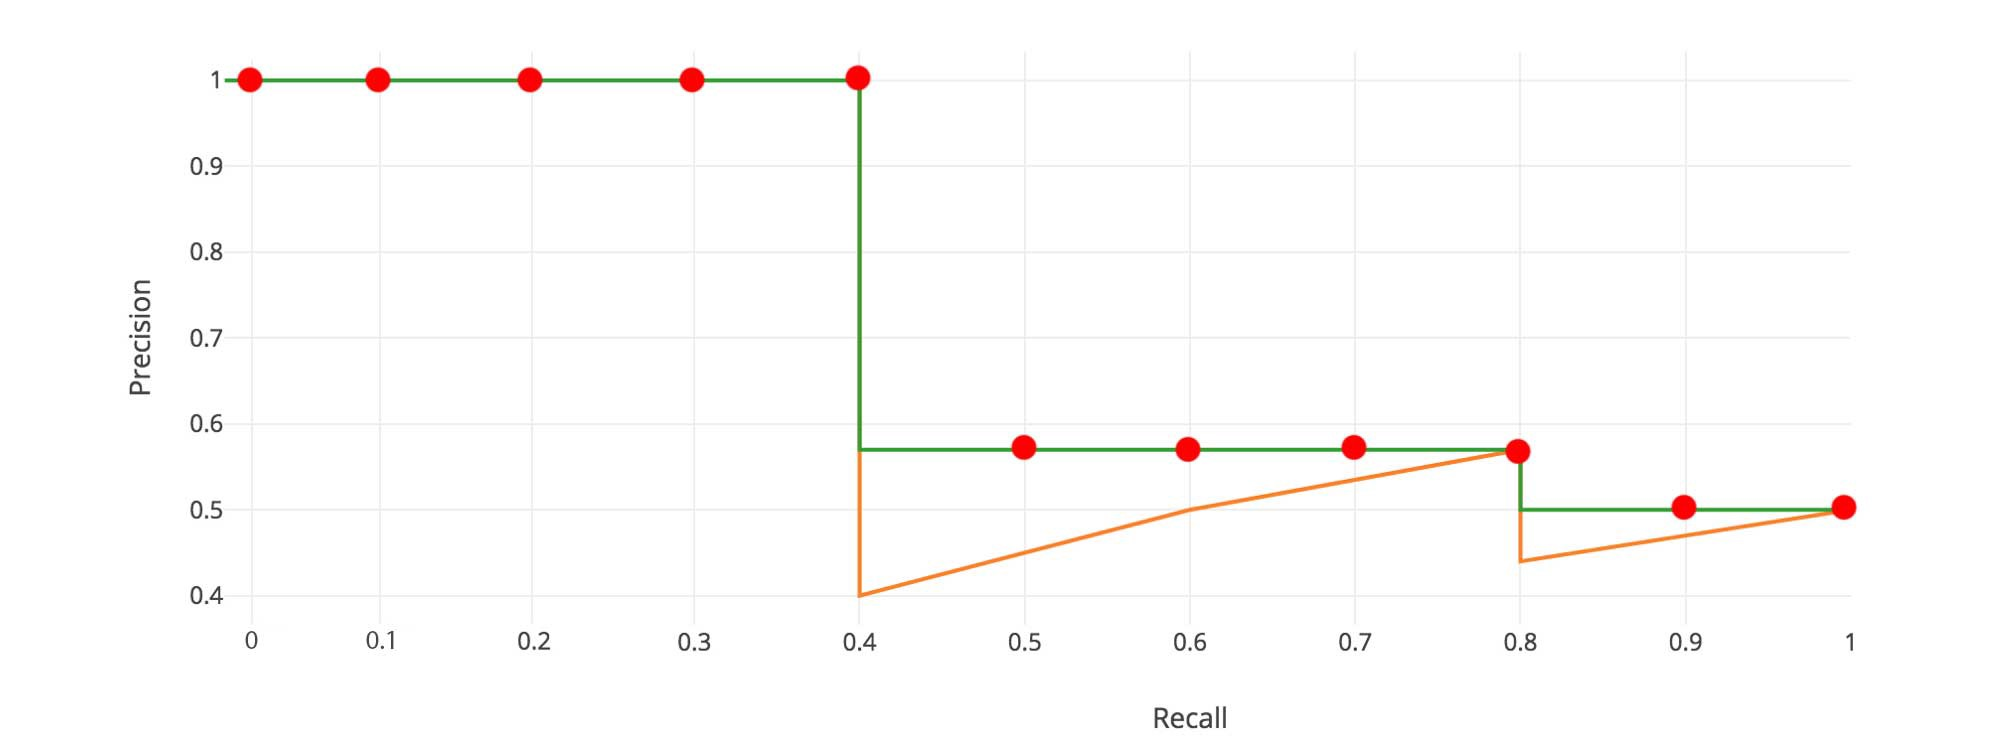
\includegraphics[width=12cm]{Bilder/map_graph2.png}} 
	\caption[Berechnung mAP]{Berechnung mAP \cite{JonathanHui.20180307}} 
	\label{map}
\end{figure} 

Im Graphen ist meist ein klassisches \glqq Zick-Zack\grqq{} Muster zu erkennen (siehe Abbildung \ref{map}). Dieses Muster wird geglättet, indem nach jedem Einbruch für jeden \textit{Recall} Wert der maximale \textit{Precision} Wert rechts des aktuellen \textit{Recalls} übernommen wird. Wird anschließend das diskrete Integral über alle \textit{Recall} Werte gebildet, so ergibt sich der \textit{Average Precision} Wert für eine zu klassifizierende Kategorie. Der Mittelwert der  \textit{Average Precisions} über alle Klassifikationskategorien hinweg ergibt letztendlich den \textit{mAP} Wert \cite{JonathanHui.20180307}. 
